\documentclass[a4paper]{scrartcl}
\usepackage[ngerman]{babel}
\usepackage[utf8]{inputenc}
\usepackage{geometry}                		             		
\usepackage{graphicx}
\usepackage{amsmath}										
\usepackage{amssymb}
\usepackage{subfigure}
\usepackage{here}
\setkomafont{sectioning}{\bfseries}	

\title{Widerstandsmessung am Halbleiter}
\author{Nora Salgo, Manuel Sommerhalder, Fabian Stäger}
		
\begin{document}
\begin{titlepage}
	\centering
	
\includegraphics[width=0.5\textwidth]{uzh.png}\par\vspace{1cm}
	\vspace{1cm}
	{\Large Praktikumsbericht Festkörperphysik\par}
	\vspace{1.5cm}
	{\huge\bfseries Widerstandsmessung am Halbleiter\par}
	\vspace{2cm}
	{\Large\itshape Nora Salgo, Manuel Sommerhalder, Fabian Stäger \par\vspace{1cm}
	Assistent: Kay Waltar}
	\vfill
	

	\vfill

% Bottom of the page
	{\large \today\par}
\end{titlepage}



\section{Physikalischer Hintergrund}
\label{ch:Physik}

Für das Experiment wird der Widerstand einer Siliziumprobe bei verschiedenen Temperaturen gemessen. Bei reinem Silizium handelt es sich um einen intrinsischen Halbleiter. Somit besteht die Ladungsträgerdichte zu gleichen Teilen aus einem Elektronenanteil $n$ und einem Lochanteil $p$.
Die elektrische Leitfähigkeit eines Halbleiters ist gegeben durch die Formel
\begin{equation}
\label{eq:sigma}
\sigma = ne\mu_e + pe\mu_h,
\end{equation}
wobei $\mu_e$ und $\mu_h$ jeweils die Mobilität der Elektronen- bzw. Loch-Beiträge ist. Diese ist leicht temperaturabhängig. Die Elektronenladungsdichte $n$ errechnet sich aus der Formel
\begin{equation}
n = \int_{E_c}^{\infty} D_e(E) f_e(E) dE
\end{equation}
mit der Zustandsdichte
\begin{equation}
D_e(E) = \frac{1}{2 \pi^2} \left(\frac{2 m_e}{\hbar^2}\right)^{3/2} (E - E_c)^{1/2}
\end{equation}
($m_e$ ist die effektive Masse, $\hbar$ die reduzierte Planck-Konstante und $E_c$ die niedrigste Energie des Leitungsbandes) und der Fermi-Dirac-Statistik
\begin{equation}
f(E,T) = \frac{1}{\exp \left(\frac{\mu - E}{k_B T}\right) + 1}
\end{equation}
($\mu$ ist hier das chemische Potential), was sich mit der Näherung $mu - \epsilon >> k_B T$ integrieren lässt zu
\begin{equation}
n = 2 \left(\frac{m_e k_B T}{2 \pi \hbar^2}\right)^{3/2} \exp \left(\frac{\mu - E_c}{k_B T}\right).
\end{equation}
Ganz analog errechnet sich die Lochdichte mit derselben Näherung zu
\begin{equation}
p = 2 \left(\frac{m_h k_B T}{2 \pi \hbar^2}\right)^{3/2} \exp \left(\frac{E_v - \mu}{k_B T}\right)
\end{equation}
($E_v$ ist die höchste Energie des Valenzbandes). Das Produkt von $n$ und $p$ ist somit nur von der Temperatur abhängig:
\begin{equation}
np = 4 \left(\frac{k_B T}{2 \pi \hbar^2}\right)^{3} (m_e m_h)^{3/2} \exp \left(\frac{-E_g}{k_B T}\right)
\end{equation}
Dabei ist $E_g = E_c – E_v$ die Energiebandlücke. Da die beiden Ladungsdichten im intrinsischen Fall gleich gross sind, lassen sie sich durch Folgende Formel in Abhängigkeit der Bandlücke und der Temperatur beschreiben:
\begin{equation}
n = p = 2 \left(\frac{k_B T}{2 \pi \hbar^2}\right)^{3/2} (m_e m_h)^{3/4} \exp \left(\frac{-E_g}{2 k_B T}\right)
\end{equation}
Der spezifische Widerstand ist somit nach einsetzen in Formel \ref{eq:sigma}
\begin{equation}
\rho = \frac{1}{\sigma} = \frac{1}{2 (\mu_e + \mu_h)e} \left(\frac{k_B T}{2 \pi \hbar^2}\right)^{-3/2} (m_e m_h)^{-3/4} \exp \left(\frac{E_g}{2 k_B T}\right)
\end{equation}
Der elektrische Widerstand ist somit
\begin{equation}
\label{eq:Endloesung}
R = A(T) T^{-3/2} \exp \left(\frac{E_g}{2 k_B T}\right)
\end{equation}
mit $A(T)$ als leicht temperaturabhängigem Proportionalitätsfaktor. 

\clearpage


\section{Auswertung}

Formel \ref{eq:Endloesung} in Kapitel \ref{ch:Physik} vereinfacht sich im Temperaturbereich des Experiments näherungsweise zu:
\begin{equation}
\label{eq:Rexp}
R \approx B \exp \left(\frac{E_g}{2 k_B T}\right)
\end{equation}
mit einer thermostatischen Proportionalitätskonstante $B$, da die Temperaturabhängigkeit der Exponentialfunktion sehr gross gegenüber dem Beitrag von $T^{-3/2}$ und den Mobilitäten $\mu_e$ und $\mu_h$ ist.
\\
Der Logarithmus der Gleichung \ref{eq:Rexp} ist dann:
\begin{equation}
\label{eq:Rlog}
\ln(R) = \ln (B) + \frac{E_g}{2 k_B} T^{-1}
\end{equation}

Aufgrund der linearen Abhängigkeit von $T^{-1}$ ist es sinnvoll, die Messwerte in einem Plot mit $T^{-1}$ in der x-Achse und ln$(R)$ in der y-Achse darzustellen. Der dadurch entstandene Graph ist grösstenteils näherungsweise linear. Bei kleinen Temperaturen bzeziehungsweise grossem $T^{-1}$ scheitert die Näherung, die in Formel \ref{eq:Rexp} gemacht wurde. Die Steigung $a$ eines linearen Fits durch den näherungsweise linearen Bereich hängt aufgrund von Gleichung \ref{eq:Rlog} direkt mit der Bandlücke zusammen:
\begin{equation}
\label{eq:bandgap}
a = \frac{E_g}{2 k_B} \quad \Rightarrow \quad E_g = 2 k_B a
\end{equation}

Dies wurde einmal für die Messung während des Aufheizens der Probe und einmal für die Messung während des Abkühlens durch:
\\
\begin{figure}[H]
\centering
    \subfigure{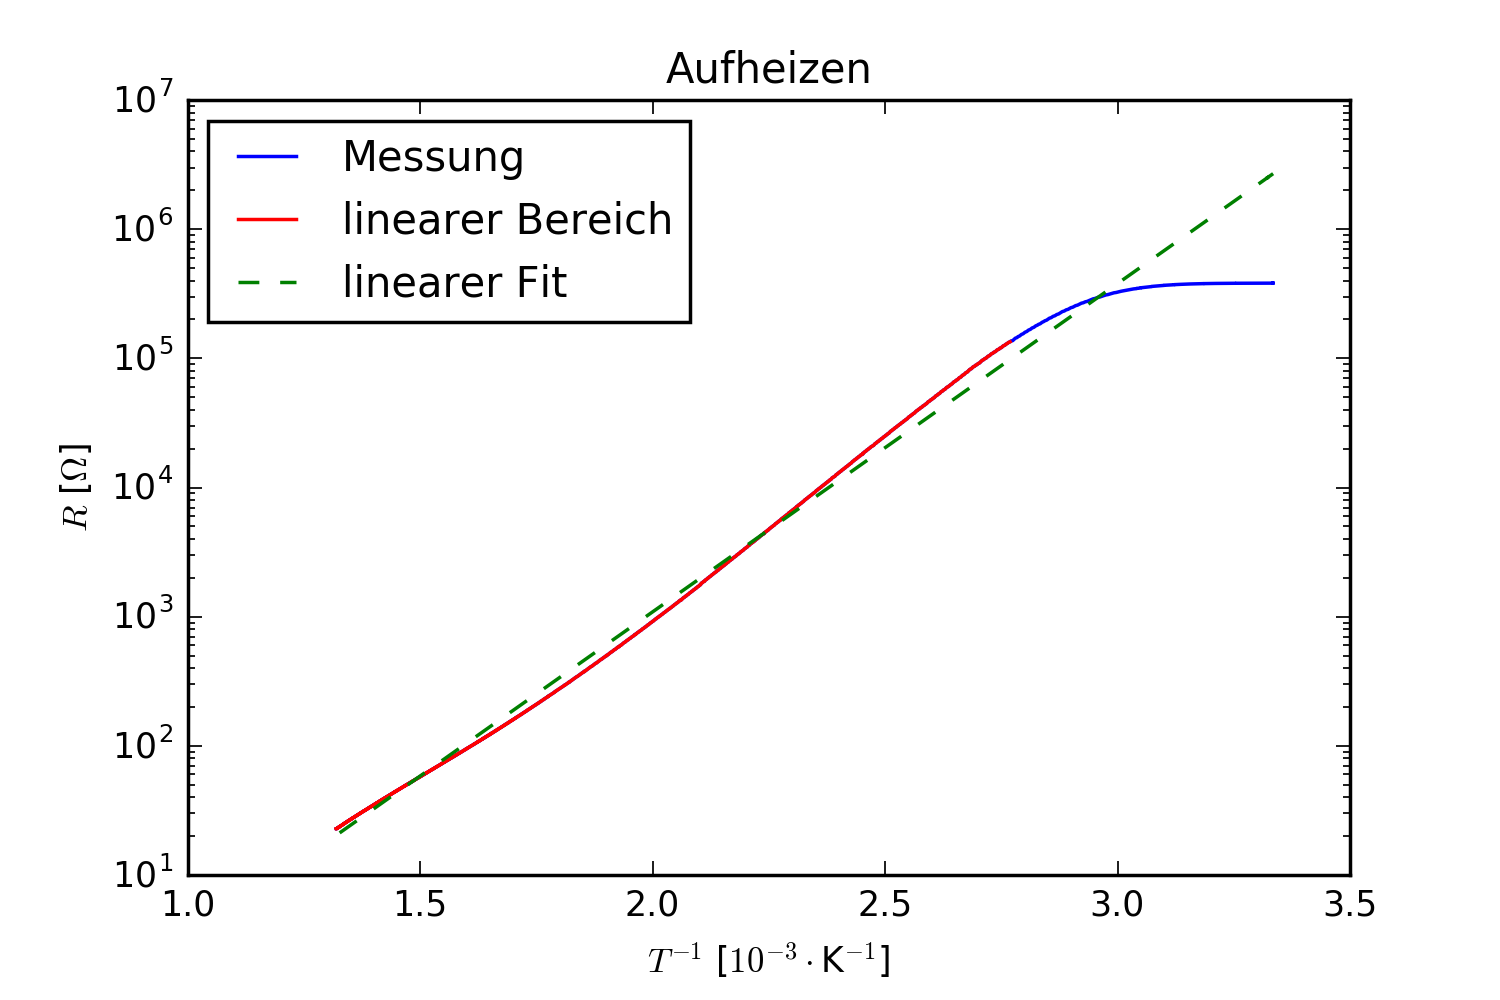
\includegraphics[width=0.45\textwidth]{temp_heat.png}}
    \subfigure{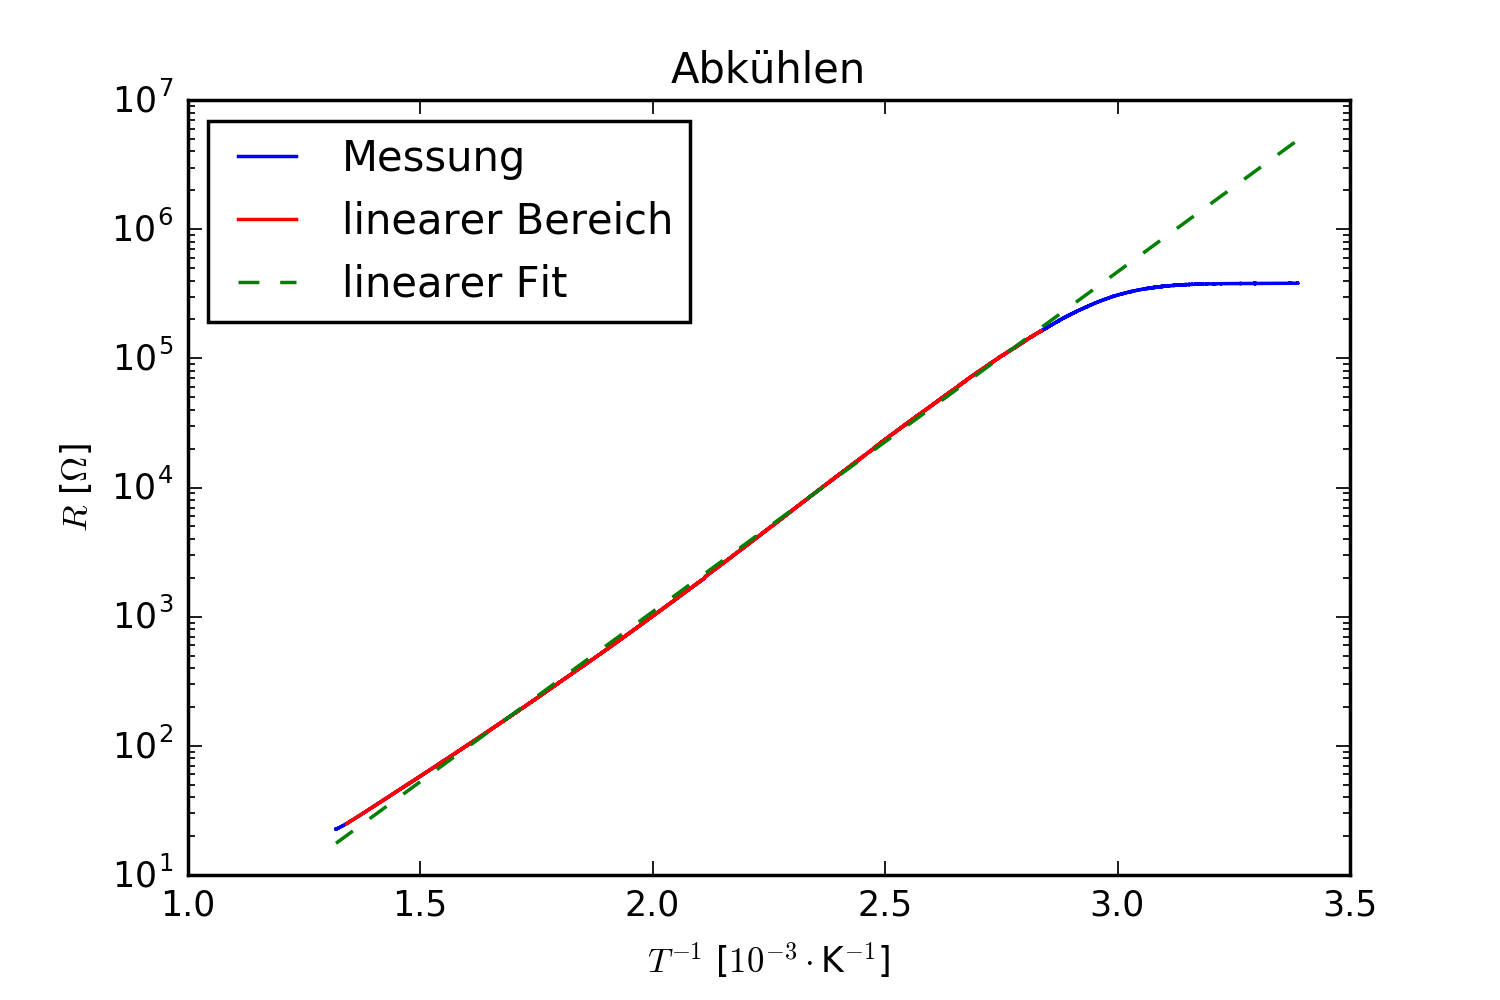
\includegraphics[width=0.45\textwidth]{temp_cool.png}}
\caption{Linearer Fit durch den näherungsweise linearen Bereich der ln$R$($T^{-1}$)-Kurve für die Messung während des Aufheizens links und Abkühlens rechts}
\end{figure}

Der rot eingefärbte Bereich der Messkurve steht für denjenigen Bereich, den wir als näherungsweise linear angenommen haben. Der lineare Fit in der Messung während des Aufheizens hat eine Steigung von $a_1$ = (5854$\pm$7)K und einen y-Achsenabschnitt von $b_1$ = -4.716$\pm$0.012. Beim Abkühlen beträgt die Steigung  $a_2$ = (6061$\pm$1)K und der y-Achsenabschnitt $b_2$ = -5.130$\pm$0.003.
\\
Erstere Messung führt sodann nach Formel \ref{eq:bandgap} zu einer Bandlücke von $E_{g,1}$ = (1.0089$\pm$0.0012)eV und letztere zu $E_{g,2}$ = (1.0446$\pm$0.0002)eV. Hier muss berücksichtigt werden, dass die angegebene Unsicherheit direkt aus dem linearen Fit kommt und keine tiefere Bedeutung hat.





\end{document}  